\chapter{Early flood warning tool}
\label{chp:flood_warning_system}


An \textit{early flood warning tool} in an essential component of an \textit{early flood warning system}.
An early flood warning system has to be understood as an integrated system of tools and plans to detect and respond to flood emergencies \autocite{icimod_early_2018}.
This can be managed by the community themselves and if designed, implemented and operated correctly can make the difference between tragedy and survival.

Such systems have already been installed in various endangered regions in the world.
After the major flooding of July 2014, the city of Altstätten in the canton of St. Gallen made the decision to install one.
The system installed uses cameras, sensors and level meters to gather data and information about the current situation \autocite{st._galler_tageblatt_altstatten_2017}.
When the value of certain parameters exceed the given threshold, a dangerous situation is recognized and the alarm signal is sent.

Three years after the installation of the system an alarm rings in the middle of the night.
Firemen go immediately into action in order to install temporary measures to fight against the water.
A couple of hours later the torrent overflows at several points and the city gets flooded.
Damages are less severe than last time, especially thanks to the temporary measures installed, but possibly they could have been reduced even more.

Crucial in order to limit the damages is the intervention time before the actual flooding occurs.
The earlier the dangerous situation can be detected the more time is available to the population and authorities to get ready and set up different types of temporary mitigation measures.
Systems based on sensors monitoring the evolution of the current situation in the upper part of the catchment are quite reliable but do not allow for long anticipation time. 

Numerical simulations can be run with meteorological forecast data and approximate soil saturation conditions in order to obtain early predictions of the event outcome.
However, the big advantage of predicting with that much anticipation is partially lost due to the duration of such simulations.
Accurate meteorological forecasts are available only few hours before the event.
If the model require several hours to run, which is often the case to obtain accurate predictions for catchments of this extent, then the advantage of being able to run it in advance is canceled.

A possible solution to this problem is the development of an \emph{early flood warning tool} based on an \emph{ad hoc surrogate model} exploiting the catchment specific behavior.
This early flood warning tool should be able to recognize if a rain event will generate a channel discharge leading to flooding and if yes within how much time.
For this scope two different emulators are used.
The first emulator classifies a rain event based on the forecasted \emph{average rain intensity} and \emph{current soil saturation} into two groups: rain events generating discharge exceeding a chosen threshold ($Q_!$) and rain events not generating discharge exceeding the threshold.
For events exceeding the threshold a second emulator is developed.
This predicts the time the rain event will need to produce the threshold discharge $Q_!$ at the outlet of the catchment.


\section{Methodology}

In order to run the simulations necessary for building the \textit{emulator}, a synthetic topography was produced.
The synthetic topography, in comparison with a real one, has the advantage of having a much smoother surface.
This ensures convergence of the solution at lower grid resolution, reducing therefore the simulation runtime.
The procedure to follow in order to build the \textit{emulator} with a real topography would be exactly the same.

The synthetic topography was produced using the software \textit{Octave 4.2.1} \seba{how to cite this?} \autocite{octave_community_gnu_2018} and the developed package \textit{fswof2d} \seba{cite it? how?} in order to export it to a format compatible with \textit{FullSWOF\_2D-v.1.07.00} \autocite{delestre_fullswof:_2014} \seba{put the citation every time that it is mentioned?}.
The generated topography is visible in Fig. \ref{fig:topography}.
It represents a catchment of $\SI{2}{\kilo\meter} \times \SI{2}{\kilo\meter}$ composed of a sloping plane with three Gaussian bumps on the top.
The Gaussian bumps have different heights and widths and generate a \emph{Y-shaped channel} which extends from the upper and left boundary down to the lower boundary.
A paraboloid was added to the plane to promote the accumulation of water in the channel.

In order to produce the dataset required for building the emulator \num{50} simulations were run with different combinations of \emph{rain intensity} ($I$) and \emph{initial soil saturation} ($\theta_i$)
Tab. \ref{tab:simulations_parameters} summarizes the parameters set and kept constant for all simulations.
The parameters marked with * are those \emph{spatially distributed}, meaning that a different value could be set for every cell by loading a matrix of values with the same size of the domain.




\begin{figure}[htpb]
  \centering
  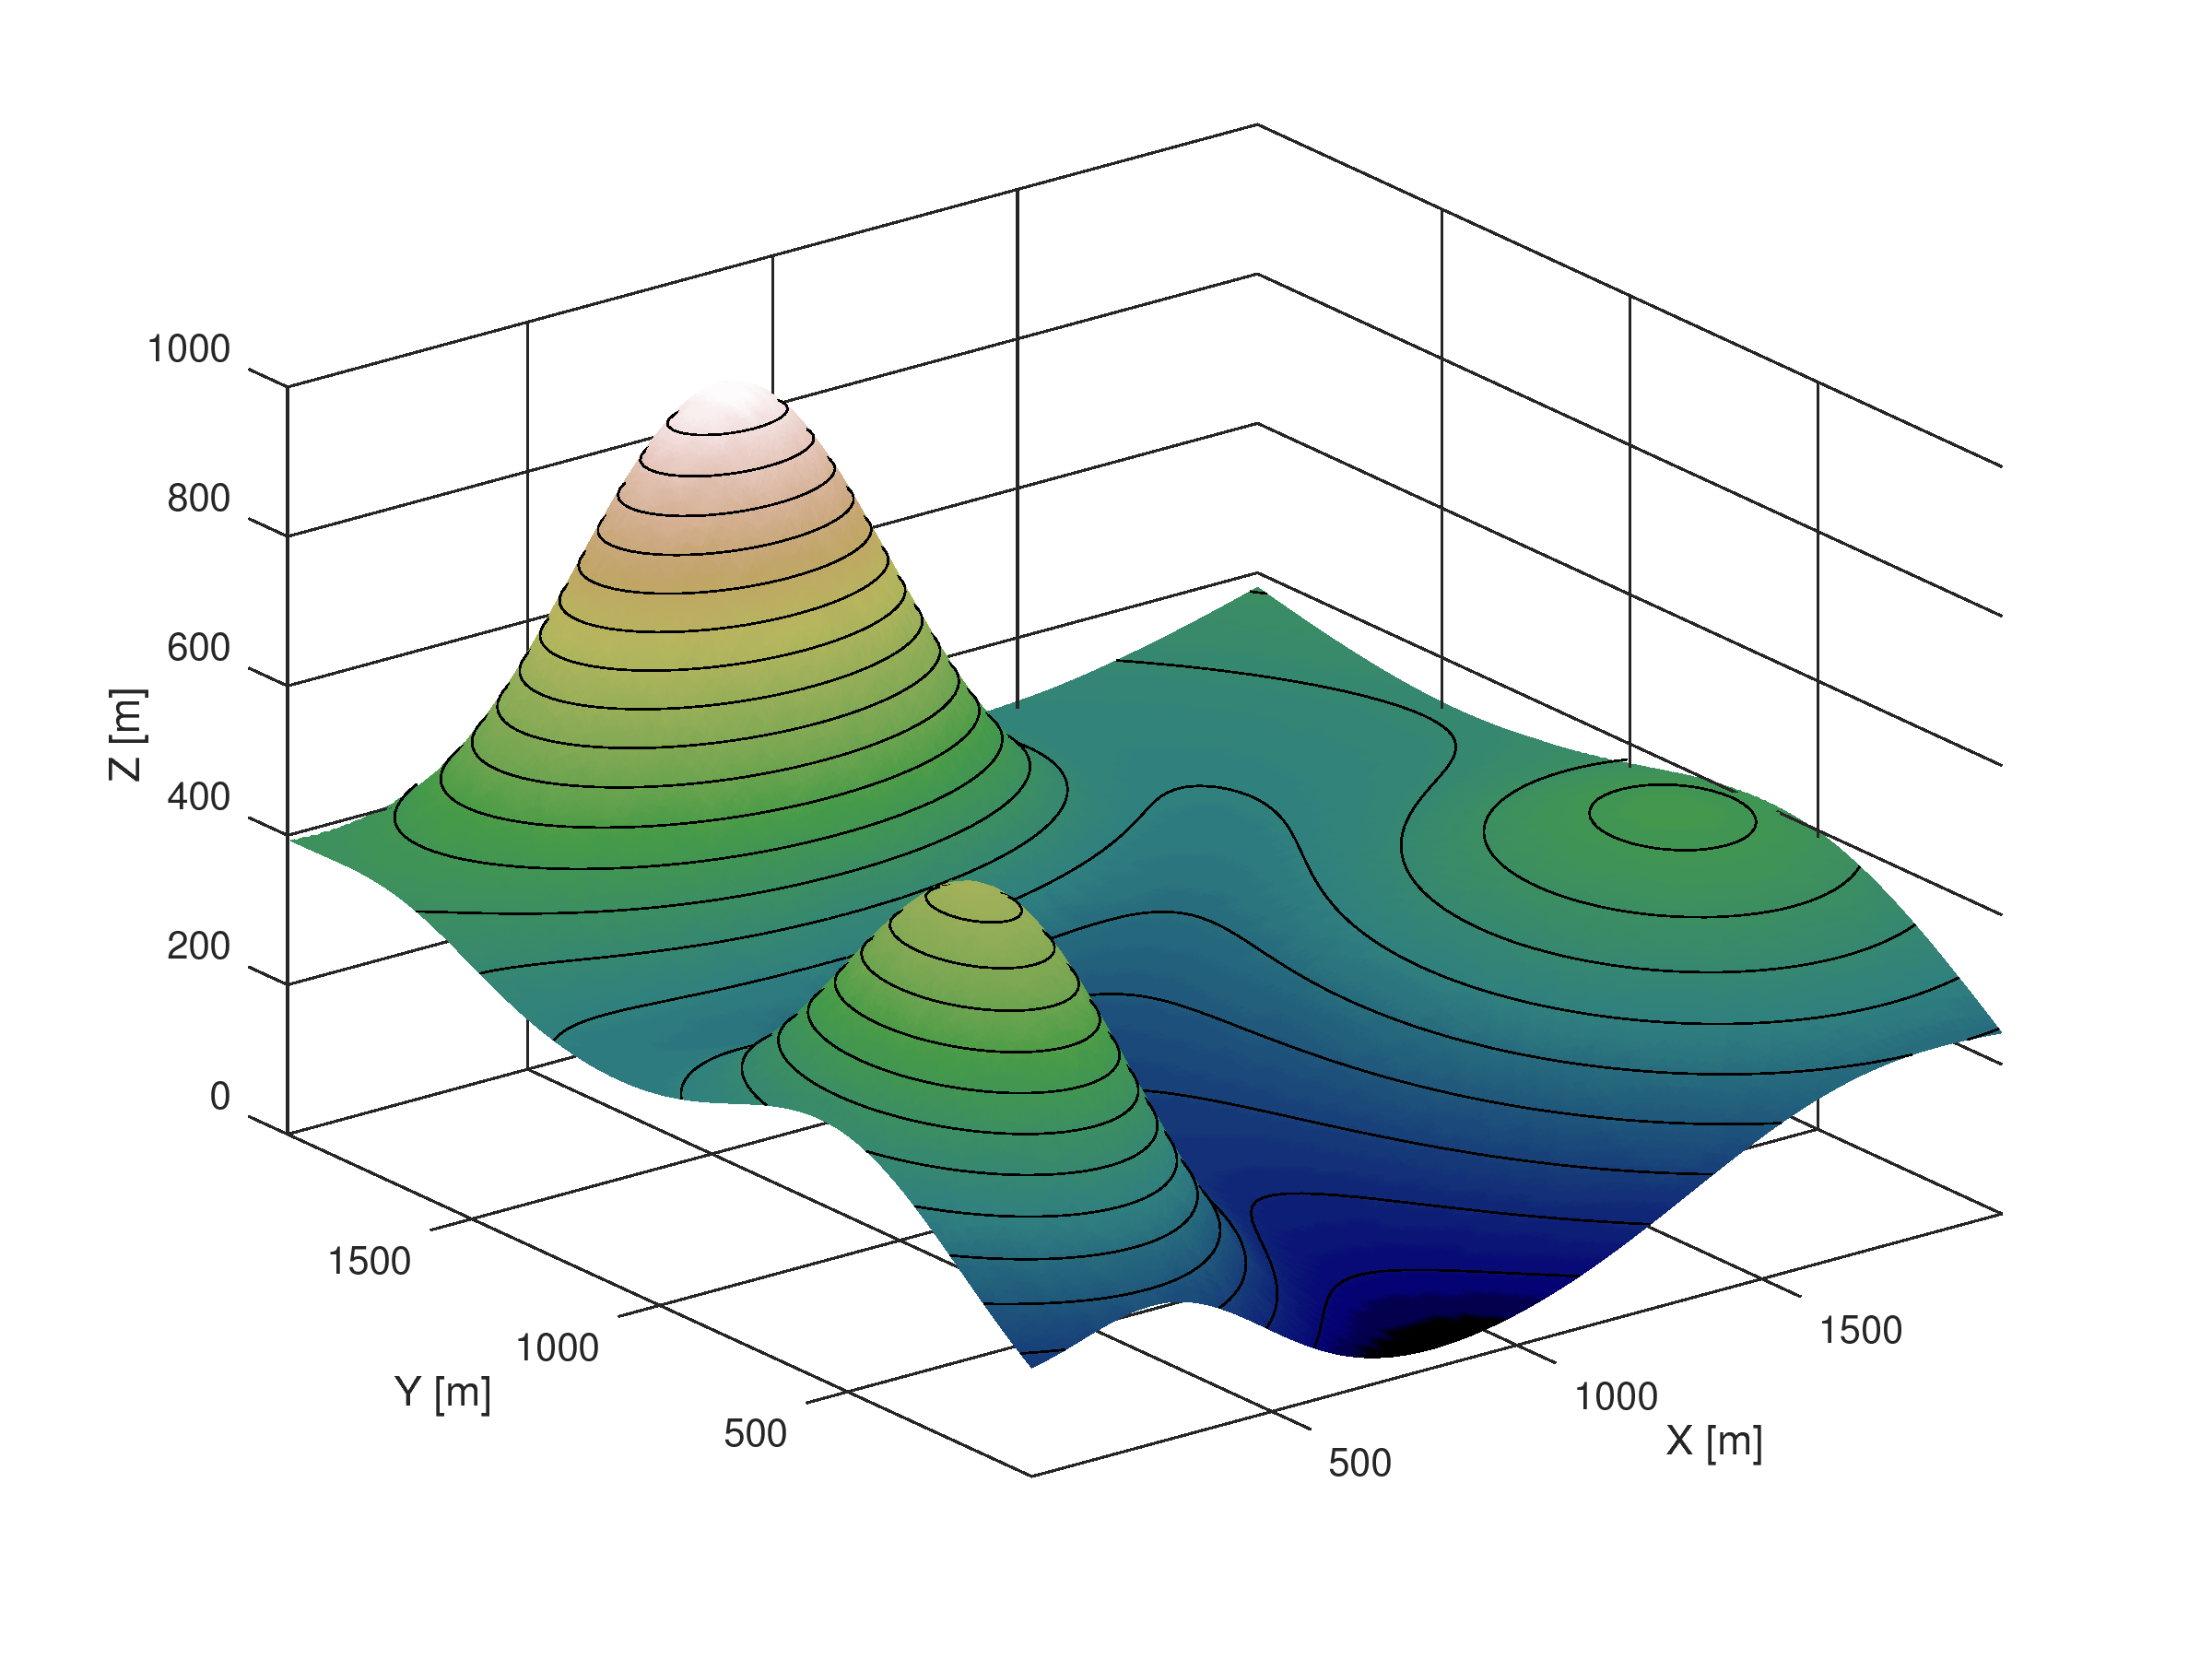
\includegraphics[width=0.7\textwidth]{../../../img/topography.png}
  \caption{Synthetic topography composed of three Gaussian bumps on a sloping plane.}
  \label{fig:topography}
\end{figure}

\begin{table}[htpb]
  \centering
  \caption{Parameters and setting fixed for all simulations.}
  \label{tab:simulations_parameters}
  \begin{threeparttable}
    \begin{tabular}{lrl}
      \toprule
      \textbf{Parameter} & \textbf{Value} & \textbf{Units} \\
      \midrule
      Domain x-length                          &    $2'000$           & \si{\meter}   \\
      Domain y-length                          &    $2'000$           & \si{\meter}   \\
      Number of cells x                        &    $100$             & --   \\
      Number of cells y                        &    $100$             & --   \\
      Friction coefficient\tnote{*}            &    $0.03$            & \si{s.m^{-1/3}}\\
      Crust thickness\tnote{*}                 &    $1$               & \si{\meter}\\
      Crust hydraulic conductivity\tnote{*}    &    $2\cdot 10^{-6}$  & \si{\meter\per\second}\\
      Soil hydraulic conductivity\tnote{*}     &    $2\cdot 10^{-6}$  & \si{\meter\per\second}\\
      Soil suction head\tnote{*}               &    $0.09$      & \si{\meter}\\
      Soil maximum infiltration rate\tnote{*}  &    $19.8$      & \si{\milli\meter\per\hour}\\
      \bottomrule
    \end{tabular}
    \begin{tablenotes}
      \item[*] Parameters spatially distributed.
    \end{tablenotes}
  \end{threeparttable}
\end{table}



\section{Results}

